\documentclass[11pt,a4paper]{article}
\usepackage[utf8]{inputenc}
\usepackage[T1]{fontenc}
\usepackage[margin=2.5cm]{geometry}
\usepackage{amsmath,amssymb}
\usepackage{graphicx}
\usepackage{booktabs}
\usepackage{siunitx}
\usepackage{microtype}
\usepackage{float}
\usepackage{xcolor}
\usepackage[font=small,labelfont=bf]{caption}
\usepackage[authoryear,round]{natbib}
\usepackage[colorlinks=true,linkcolor=blue!50!black,citecolor=blue!50!black,urlcolor=blue!50!black]{hyperref}
\usepackage[capitalise,noabbrev]{cleveref}

\graphicspath{{../figures/}}

\title{Lighting a Line-Scan Camera:\\ Illumination Design and Camera Calibration}
\author{Juan Carlos Chavarr\'ia Morales\\[2pt]
  \small M.Sc.\ Optimization, Hochschule Bielefeld (HSBI)\\
  \small Module \emph{Simulation optischer Systeme}, winter term 2024/25}
\date{October 2026}

\begin{document}
\maketitle

\begin{abstract}
A line-scan camera images one line of a moving surface; for a clean image, the light along that line must be as
uniform as possible. We model the illumination of a laboratory set-up, two rectangular light panels at the ends of
a scan line about half a metre long, and optimise their placement. Three results. First, the objective used in the
project's first scripts, the absolute standard deviation of the irradiance, is minimised by dimming the lights: a
relative measure (min/mean or standard deviation/mean) is needed. Second, at the same efficiency as the lab
geometry, a different placement of the panels raises the uniformity $U_0 = \min/\text{mean}$ along the line from
0.80 to 0.95, and the Pareto front shows how much uniformity each gain in efficiency costs; in our reading of the
geometry, the lab panels also slightly enter the camera's field of view. Third, from seven line-scan images of a
checkerboard target we calibrate the camera geometrically: \SI{0.120}{mm} per pixel on the target, residuals of
\SI{0.06}{px} once the printing errors of the target ($\pm$\SI{0.14}{mm}) are estimated jointly. The same images
cannot validate the illumination model: the light areas are saturated. We give the measurement protocol that
would.
\end{abstract}

% =====================================================================================================================
\section{The set-up}

The scan line is the $x$-axis of the inspection plane $z = 0$. A line-scan camera with 4096 pixels looks down from
$z_c = \SI{606.5}{mm}$; its field of view on the target is \SI{491}{mm} (\cref{sec:calibration}). Two light panels
of $\SI{210}{mm} \times \SI{510}{mm}$ are placed symmetrically at the ends of the line: centres at $x = \pm W/2$,
$W = \SI{480}{mm}$, height $z_0 = \SI{209}{mm}$, tilted by $\theta = 15^\circ$ (\cref{fig:design}, left).
The project asked how to place such lights for a uniform line, and how to calibrate the camera.

% =====================================================================================================================
\section{Models and the measure of uniformity}

\paragraph{Point sources.} The first model of the project replaced each light by an isotropic point source of power
$P$ at $(\pm d, z_s)$; with the inverse-square law and the cosine of incidence,
\begin{equation}
  E(x) = \frac{P z_s}{\left((x-d)^2 + z_s^2\right)^{3/2}} + \frac{P z_s}{\left((x+d)^2 + z_s^2\right)^{3/2}}.
\end{equation}

\paragraph{Panels.} For the lab, each panel is a generalised Lambertian emitter \citep{Moreno2008}: a surface element
$\mathrm dA$ at $\mathbf q$ with normal $\mathbf n$ sends to the point $\mathbf p$ on the line
\begin{equation}
  \mathrm dE = L_0 \, \frac{\cos^m\vartheta_s \, \cos\vartheta_r}{\lVert \mathbf p - \mathbf q\rVert^2}\, \mathrm dA,
\end{equation}
with $\vartheta_s$ the emission angle at the panel, $\vartheta_r$ the incidence angle on the plane, and $m = 1$ for a
diffuse (Lambertian) panel, $m > 1$ for a more directed one. The irradiance is the integral over both panels,
computed by Gauss--Legendre quadrature ($8 \times 12$ nodes per panel are converged to $10^{-6}$; the $3 \times 3$
nodes of the original notebook give errors of up to \SI{6}{\percent}).

\paragraph{Uniformity.} We use the overall uniformity of lighting standards, $U_0 = E_{\min}/\bar E$, and the
coefficient of variation $\mathrm{CV} = \sigma_E / \bar E$. Both are relative. The first scripts of the project
minimised the absolute standard deviation $\sigma_E$ over the powers, the height and the distance of two point
sources. Since $\sigma_E$ is proportional to the power, the optimiser lowers the power to its bound and moves the
lights as far away as allowed: the ``optimum'' sits on the bounds and has $U_0 = 0.74$. Minimising CV instead gives
$U_0 = 0.89$ for the same bounds (\cref{fig:points}). The same issue reappears in any design problem in which the
objective scales with the light: uniformity must be measured relative to the mean, and the light output treated as
a separate goal.

\begin{figure}[t]
  \centering
  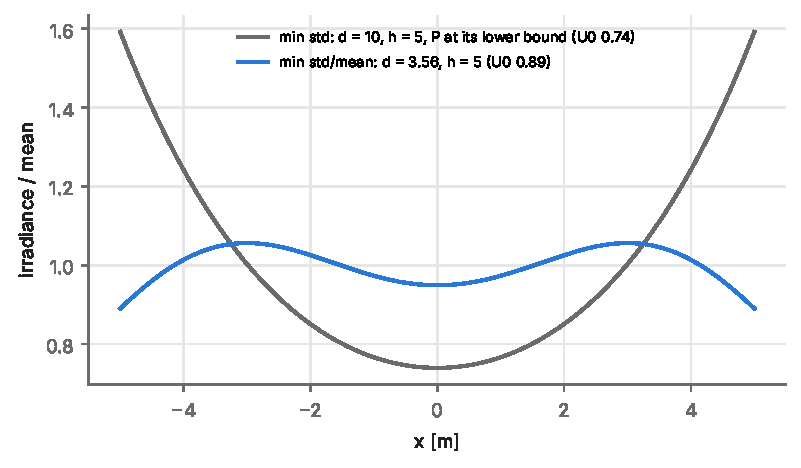
\includegraphics[width=0.7\linewidth]{point_sources.pdf}
  \caption{Two point sources on a \SI{10}{m} line: the optimum of the absolute standard deviation (the sources dimmed
    and moved to the bounds) and of the relative one.}
  \label{fig:points}
\end{figure}

% =====================================================================================================================
\section{Designing the illumination}\label{sec:design}

Over the field of view, the lab set-up has $U_0 = 0.80$: the line is \SI{20}{\percent} darker in the middle than on
average (\cref{fig:design}, right). Tilting the panels further towards the centre helps: at $25^\circ$, $U_0 = 0.83$
with the same light on the line. In our reading of the geometry, the inner edges of the lab panels reach about
\SI{1}{cm} into the cone in which the camera sees the line; from $25^\circ$ on they are out of it. This should be
checked on the real set-up.

\begin{figure}[t]
  \centering
  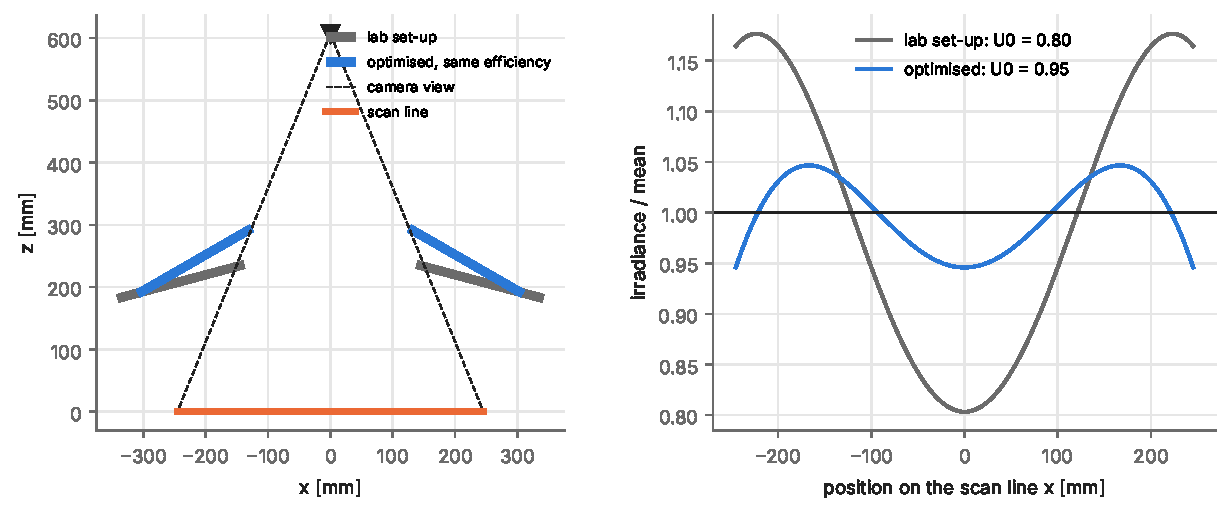
\includegraphics[width=\linewidth]{design.pdf}
  \caption{Left: the lab set-up and the optimised placement of the panels at the same efficiency (section through
    the scan line; the panels extend \SI{510}{mm} across it), with the camera's view of the line. Right: irradiance
    along the line, normalised by its mean.}
  \label{fig:design}
\end{figure}

\paragraph{Optimisation.} What can be chosen is the geometry: distance $W$, height $z_0$ and tilt $\theta$. Two goals
conflict: uniformity, and efficiency, i.e.\ how much of the emitted flux reaches the line (mean irradiance per unit
emitted flux, relative to the lab set-up). We maximise $U_0$ for a range of minimum efficiencies, with the constraint
that the panels stay out of the camera's view, by differential evolution with a local polish. \Cref{tab:design,fig:pareto}
give the Pareto front. At the efficiency of the lab set-up, $U_0$ rises from 0.80 to 0.95 (panels closer together,
higher and tilted by $30^\circ$); a uniformity of 0.97 to 0.99 is possible at 80 to \SI{45}{\percent} of the
efficiency; and \SI{20}{\percent} more efficiency costs uniformity down to 0.85. More directed emitters ($m = 3$)
give a similar front, slightly lower at high efficiency.

\begin{table}[t]
  \centering\small
  \caption{Lab set-up and optimised designs (Lambertian panels, field of view \SI{491}{mm}). Efficiency relative to
    the lab set-up.}
  \label{tab:design}
  \resizebox{\linewidth}{!}{\begin{tabular}{lrrrrrrc}
\toprule
design & $W$ [mm] & $z_0$ [mm] & $\theta$ [$^\circ$] & $U_0$ & CV & efficiency & blocks view \\
\midrule
lab set-up & 480 & 209 & 15 & 0.80 & 0.137 & 1.00 & yes \\
lab, tilt 25$^\circ$ & 480 & 209 & 25 & 0.83 & 0.115 & 1.02 & no \\ \midrule
optimum, efficiency $\ge$ 0.4 & 636 & 450 & 33 & 0.989 & 0.007 & 0.45 & no \\
optimum, efficiency $\ge$ 0.6 & 512 & 386 & 13 & 0.982 & 0.011 & 0.60 & no \\
optimum, efficiency $\ge$ 0.8 & 455 & 308 & 15 & 0.969 & 0.020 & 0.80 & no \\
optimum, efficiency $\ge$ 1.0 & 435 & 242 & 30 & 0.946 & 0.035 & 1.00 & no \\
optimum, efficiency $\ge$ 1.2 & 415 & 157 & 55 & 0.851 & 0.103 & 1.20 & no \\
\bottomrule
\end{tabular}
}
\end{table}

\begin{figure}[t]
  \centering
  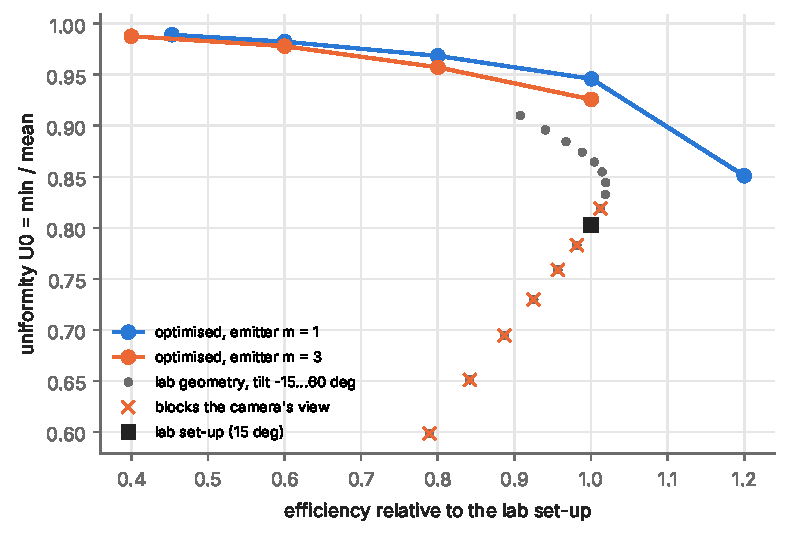
\includegraphics[width=0.65\linewidth]{pareto.pdf}
  \caption{Uniformity against efficiency: Pareto fronts of the optimised geometry, and the lab geometry with
    different tilts (crosses: the panels enter the camera's view). For $m = 3$ the efficiency is relative to the lab
    geometry with that emitter.}
  \label{fig:pareto}
\end{figure}

% =====================================================================================================================
\section{Calibrating the line-scan camera}\label{sec:calibration}

A line-scan image repeats one sensor line over time; seven images show a row of eight edges of a checkerboard target
(square size \SI{26.54}{mm}) at different positions (\cref{fig:images}). Averaging the 50 lines of an image and
locating the mid-level crossings with sub-pixel interpolation gives eight edge positions per image. Two images were
taken at the same position: their edges agree to \SI{0.024}{px} (RMS), which is the repeatability of the
measurement.

\begin{figure}[t]
  \centering
  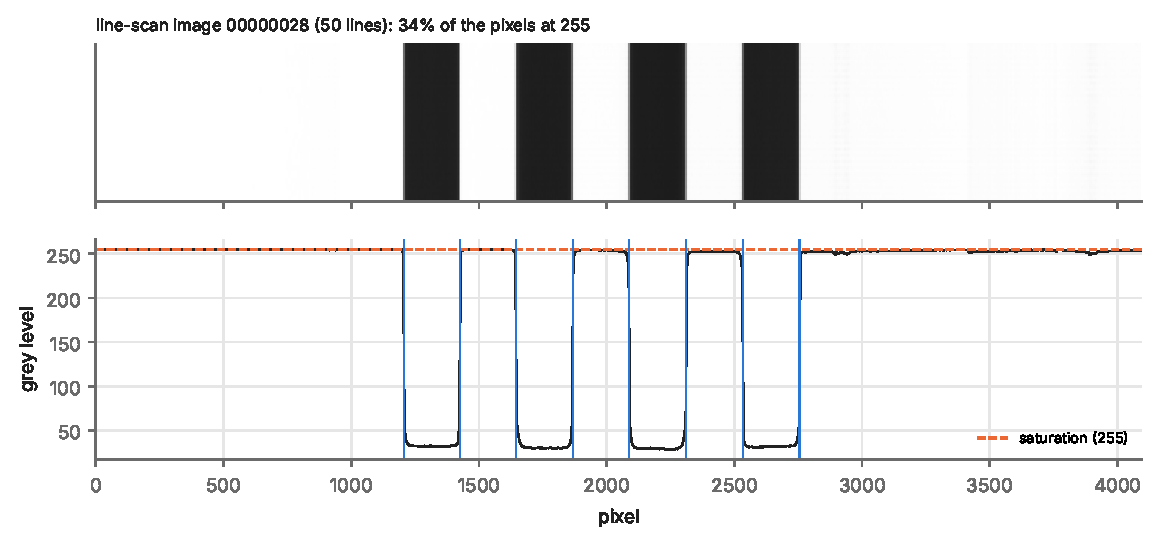
\includegraphics[width=0.9\linewidth]{images.pdf}
  \caption{A line-scan image of the target and its mean profile. The light squares and the background are saturated
    (grey level 255); blue: detected edges.}
  \label{fig:images}
\end{figure}

A line camera maps a position $X$ on a (possibly tilted) target to the pixel $u = (a + bX)/(1 + cX)$, a 1-D
projective map \citep[the general line-scan model is discussed by][]{Steger2021}. Per image, a linear map leaves
residuals of \SI{1.4}{px} (RMS) and the projective map \SI{0.6}{px} (\cref{tab:calib,fig:calib}), 25 times the
repeatability. The residual pattern, however, is the same in every image, although the target lies at different
places on the sensor: it belongs to the target, not to the camera. Estimating one deviation per edge of the target,
common to all images, together with the per-image maps, reduces the residuals to \SI{0.06}{px} for six images, about
\SI{7}{\micro m} on the target. The printed squares deviate from their nominal positions by up to \SI{0.14}{mm}
(\cref{fig:calib}, right).

\begin{table}[t]
  \centering\small
  \caption{Calibration per image: share of saturated pixels, range of the edges on the sensor, scale, and RMS
    residuals of the three models (the joint fit with target deviations excludes image 00000037, taken with a
    different exposure).}
  \label{tab:calib}
  \begin{tabular}{lrcrrrr}
\toprule
image & saturated [\%] & edges [px] & scale [px/mm] & \multicolumn{3}{c}{RMS residual [px]} \\ \cmidrule(lr){5-7}
& & & & linear & projective & + target \\
\midrule
00000028 & 34 & 1206--2755 & 8.343 & 1.22 & 0.57 & 0.048 \\
00000029 & 34 & 1199--2748 & 8.345 & 1.28 & 0.60 & 0.035 \\
00000030 & 34 & 1253--2802 & 8.348 & 1.11 & 0.60 & 0.035 \\
00000032 & 35 & 1004--2550 & 8.330 & 2.00 & 0.61 & 0.041 \\
00000033 & 34 & 1004--2550 & 8.330 & 1.99 & 0.61 & 0.042 \\
00000034 & 42 & 1402--2952 & 8.349 & 0.71 & 0.69 & 0.118 \\
00000037 & 14 & 1182--2732 & 8.346 & 1.39 & 0.77 & -- \\
\bottomrule
\end{tabular}

\end{table}

\begin{figure}[t]
  \centering
  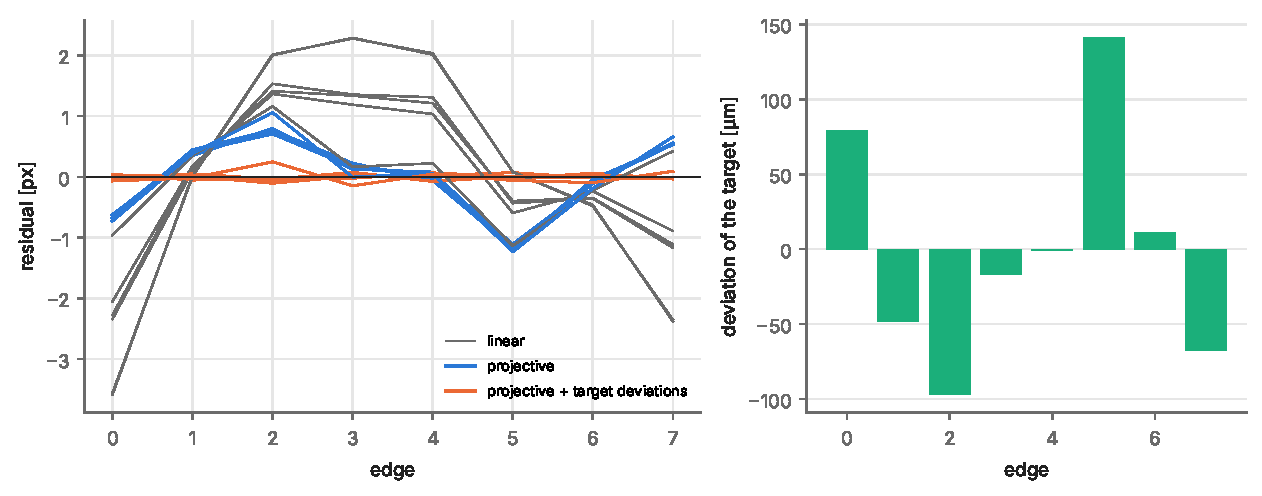
\includegraphics[width=\linewidth]{calibration.pdf}
  \caption{Left: residuals of the linear, projective and joint models for the six images with the same exposure.
    Right: estimated deviations of the target's edges from the nominal grid (the part not absorbed by a tilt or
    scale of the projective map).}
  \label{fig:calib}
\end{figure}

\paragraph{Results.} The scale on the target is \SI{8.34}{px/mm}, i.e.\ \SI{0.120}{mm} per pixel and a field of view
of \SI{491}{mm}; across the target it changes by 0.2 to \SI{2.7}{\percent}, a sign of a slightly tilted target. Three
limits: (i) the edges cover only pixels 1000 to 2950, so lens distortion near the ends of the sensor cannot be
identified; (ii) the image taken with a different exposure (00000037) does not fit the others (\SI{0.38}{px}): in
saturated images the position of an edge depends on the exposure; (iii) the intrinsic matrix of the original
notebook came from an area-camera calibration routine applied to these images. Its vertical entries have no meaning
for a line-scan camera (the vertical axis is time), and its focal length (\SI{4804}{px}) together with the measured
scale implies a working distance of \SI{576}{mm}, \SI{5}{\percent} less than the camera height used in the model.

% =====================================================================================================================
\section{What has not been validated}

The images were meant to validate the illumination model as well, by fitting the emission parameters of the panels
to the measured profile. They cannot: in six of them 34 to \SI{42}{\percent} of the pixels are at the maximum grey level (\SI{14}{\percent} in the seventh), the
light areas carry no information about the irradiance, and any uniformity computed from them is close to 1 by
construction. The original notebook also maximised the uniformity over the emission parameters instead of fitting
them: emission is a property of the panels, to be measured; only the geometry is to be optimised. A validation
would need:
\begin{enumerate}
  \item a diffuse white target (e.g.\ PTFE) without pattern, imaged with exposure and gain set so that the brightest
    pixel stays below about \SI{80}{\percent} of the range, plus a dark frame;
  \item the camera's flat-field response (vignetting), measured once under uniform light, divided out;
  \item a least-squares fit of the emission exponent $m$ and the scale $L_0$ to the profile, and only then the
    design optimisation of \cref{sec:design}, followed by a measurement at the optimised geometry.
\end{enumerate}

% =====================================================================================================================
\section{Main changes}

\begin{table}[H]
  \centering\small
  \caption{Main changes with respect to the original scripts and notebooks.}
  \begin{tabular}{p{0.2\linewidth}p{0.34\linewidth}p{0.36\linewidth}}
    \toprule
    & original & this version \\
    \midrule
    Uniformity & absolute standard deviation (minimised by dimming); later min/mean on saturated data & $U_0$ and CV
      on the model; efficiency as a separate goal \\
    Panel model & beam profile $1/(1 + (r/a)^2)^b$ without cosines, $3 \times 3$ quadrature & generalised Lambertian
      emitter with emission and incidence cosines, converged quadrature \\
    Optimisation & of the emission parameters (properties of the hardware) & of the geometry, with a view constraint;
      Pareto front uniformity vs efficiency \\
    Calibration & area-camera routine on line-scan images & 1-D projective model per image, joint estimation of the
      target's printing errors \\
    Validation & claimed from saturated images & not possible with these images; protocol given \\
    Code & notebooks & package, scripts for every table and figure, tests on synthetic data \\
    \bottomrule
  \end{tabular}
\end{table}

% =====================================================================================================================
\section{Conclusions}

\begin{enumerate}
  \item Uniformity has to be measured relative to the mean light level; minimising the absolute spread optimises the
    lights away.
  \item For the lab panels, a different placement (closer together, higher, more tilted) raises the uniformity along
    the line from 0.80 to 0.95 without losing light; the uniformity--efficiency trade-off is quantified by the Pareto
    front. The lab panels seem to touch the camera's view and should be checked.
  \item The line-scan camera is calibrated to \SI{0.120}{mm} per pixel with residuals of \SI{0.06}{px}, once the
    printing errors of the target are estimated; a target spanning the whole sensor would also identify lens
    distortion.
  \item The illumination model is not yet validated: the existing images are saturated. A measurement with a plain
    white target at lower exposure is the next step, and the deciding one for whether the idea is worth pursuing.
\end{enumerate}

\section*{Code and data}
Code, the seven calibration images and the scripts for every table and figure: \citet{Repo}.

\bibliographystyle{plainnat}
\bibliography{references}

\end{document}
